
%(BEGIN_QUESTION)
% Copyright 2008, Tony R. Kuphaldt, released under the Creative Commons Attribution License (v 1.0)
% This means you may do almost anything with this work of mine, so long as you give me proper credit

Calculate the proper $C_v$ value for this valve, given the flow rate and pressures shown for full-open condition.  Assume the process liquid is acetic acid (specific gravity = 1.05):

$$\includegraphics[width=15.5cm]{i03219x01.eps}$$

\underbar{file i03219}
%(END_QUESTION)





%(BEGIN_ANSWER)

$C_v$ = 0.416
 
%(END_ANSWER)





%(BEGIN_NOTES)


%INDEX% Final Control Elements, valve: sizing

%(END_NOTES)


